\section{Discussion}
\label{sec:chromium-discussion}

We seek to better understand the results showing that existing approaches targeting the detection of flaky tests missed a non-negligible part (76.2\%) of fault-triggering failures by classifying them as flaky. To do so, we investigate the following aspects regarding \textit{the entire dataset}.

We first report general information about the prevalence of flaky tests and fault-revealing tests in order to have a better view of the failures occurring in each build. Then, we report the number of fault-revealing tests also found as flaky by the Chromium CI (reruns) in other builds (we further refer to them as fault-revealing flaky tests). Finally, we also check for the number of failing builds that only contain fault-revealing flaky tests. We consider these builds important since the related faults are not detected by any non-flaky test and would be missed if flaky test detectors were used.

% Figure Tests per Build
\begin{figure}[ht]
\centering
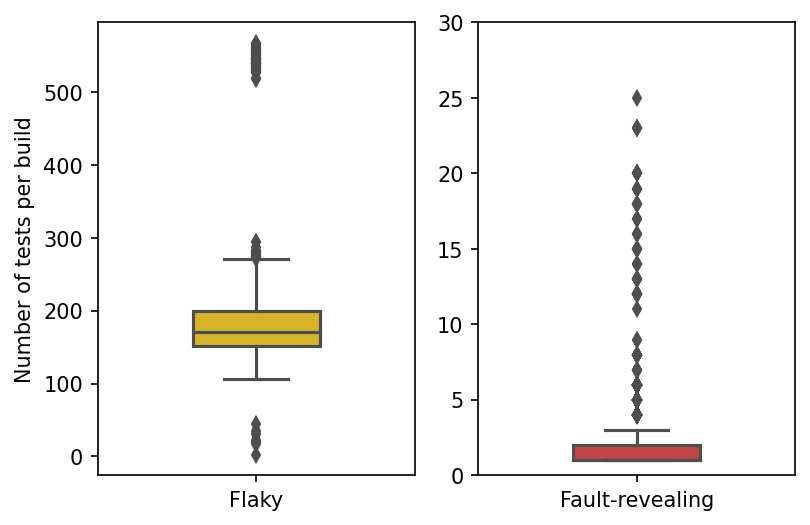
\includegraphics[width=0.6\textwidth]{figures/chromium/testsPerBuild.png}
\caption{Number of flaky tests and fault-revealing tests per build. On average, there are 250 flaky tests per build and 1 fault-revealing test per failing build.}
\label{fig:testsPerBuild}
\end{figure}

Figure~\ref{fig:testsPerBuild} shows the distribution of flaky tests and fault-revealing tests in the studied builds. We observe that there is an average of 178 flaky tests per build with a low standard deviation (41), showing that flakiness is prevalent in the Chromium CI. In the case of fault-revealing tests, taking into account all builds would result in an average number of tests close to 0 as a majority of builds are exempt from them. Thus, for better visualisation, we only considered builds containing at least one fault-revealing test (\ie failing builds). The average number of fault-revealing tests per failing build is 2.7.

The standard deviation for fault-revealing tests is 14.9 and the number of fault-revealing tests reported in one build goes up to 579 in our dataset.

\begin{table}[ht]
\caption{Number of builds containing each studied test type. All builds contain flaky tests. \nicefrac{1}{4} contain fault-revealing tests. Among the failing builds, \nicefrac{3}{4} contain only fault-revealing tests that are flaky in other builds.}
\label{table:DiscBuilds}
\centering
\begin{tabular}{c|c} 
 \toprule
 \textbf{Builds containing} & \textbf{Number} \\ [0.5ex] 
 \midrule
 Flaky tests & 10,000 \\ 
 Fault-revealing tests & 2,415 \\ 
 Fault-revealing flaky tests & 1,974 \\ 
 Exclusively fault-revealing flaky tests & 1,766 \\ 
 \bottomrule
\end{tabular}
\end{table}

Table~\ref{table:DiscBuilds} provides, for each type of test, the number of builds that contain at least one instance of this type. We note that all builds contain at least one flaky test (a test that flaked during this build). In Chromium CI, flaky tests are non-blocking and will not cause a build failure. That is, tests flaking within the build are ignored during this build. 

Developers are expected to investigate test failures only when they occur consistently across 5 reruns (resulting in a fault-revealing test). Such fault-revealing tests occur in 24.15\% of the builds (i.e. in 2,415 builds). Interestingly, 1,974 of these builds (i.e. 81.73\%) contain fault-revealing tests that flaked in previous builds, indicating that \emph{tests with a flake history should not be ignored in future builds}. Perhaps worse, in 1,766 builds \emph{all} fault-revealing tests have flaked in some previous builds, indicating that no "reliable" tests identified the fault(s).

% Figure Venn diagram
\begin{figure}[ht]
\centering
%\vspace{-0.5m}
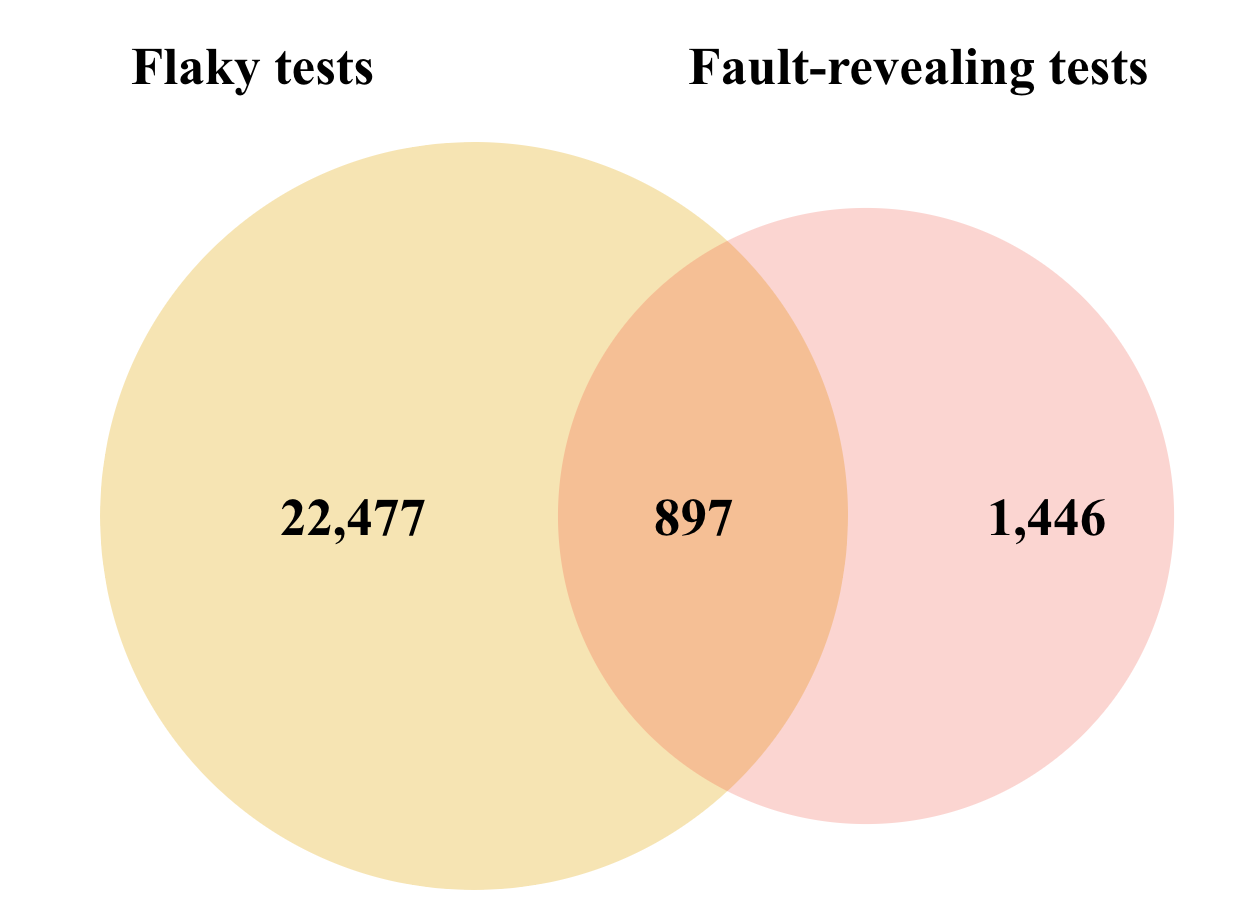
\includegraphics[width=0.5\textwidth]{figures/chromium/venn.png}
\caption{Distribution of tests in our dataset. 22,477 tests are exclusively flaky among all builds. 2,343 tests are fault-revealing, among which \nicefrac{1}{3} are flaky in other builds.}
\label{fig:venn}
\end{figure}

By investigating the status of all tests across all builds -- see Figure~\ref{fig:venn}. Among the 209,530 tests of the Chromium project, 24,820 have failed in at least one build, including 22,477 that were always flaky. Thus, 2,343 tests were fault-revealing in at least one build, i.e., they attested the presence of faults, 897 were also flaky in at least one other build. That is, \emph{38.3\% of tests that have been useful to detect faults have also a history of flakiness}.

\begin{tcolorbox}[
    left=2pt,right=2pt,top=2pt,bottom=2pt,
    arc=0pt,
    boxrule=1.2pt
]
Flakiness affects all Chromium CI builds and mixes critical (fault-revealing) signals with false (flakiness) signals. Indeed, 81.7\% of builds contain fault-revealing tests that were flaky in some previous builds, and 38.3\% of all tests flake in some builds and reveal faults in other builds. 
\end{tcolorbox}